\chapter{黑白视频着色算法}
\label{cha:3-video-color}

  本章介绍了本文中使用的所有网络、算法。第\ref{sec:3-image-color}节介绍了本文黑白图像着色的模型选择,经过验证的模型在第\ref{sec:3-video-color}节中应用到了黑白视频着色上。第\ref{sec:3-other-algorithm}节介绍了用于帧内帧间的平滑算法与非关键帧着色算法。最后\ref{sec:3-experiment}节展示了实验结果。

\section{黑白图像着色}
\label{sec:3-image-color}

  基于wGAN的架构,本文训练了几种模型用于黑白图像着色,下面介绍本文的网络结构以及相关训练参数。

\subsection{判别器网络}
\label{sec:3-image-dnet}
  
  判别器网络使用了比较常见的CNN网络,其详细参数如下:对于分辨率为64x64的图像,判别器中有4层卷积层与其对应的BN层和LeakyReLU层,每个卷积核均为4,步幅为2,边缘填充为1。这样每个卷积层都是图像分辨率减半,特征通道数翻倍。在得到4x4的特征后,再经过一个卷积核为4,步幅为1,边缘填充为0的卷积层,就得到输出的1x1的结果,即判别器给出的图像是真实的概率。
  
\subsection{生成器网络}
\label{sec:3-image-gnet}

  生成器网络是GAN中最重要的一部分,因为它的是否合适决定了最终生成器能否生成理想的结果。本文尝试了基线模型,变分自编码器与U-NET几种结构。对于着色问题而言,本文在所有的生成器网络结构中都没有使用池化层,因为池化层是通过压缩空间上的信息来降低分辨率,这样会丢失一些信息,所以本文都是通过步幅大于1的卷积层达到压缩的目的。


  \begin{enumerate}
  \item 基线模型
  
  着色问题与一般分类、回归问题的很大不同在于,着色的输入输出分辨率是一样的,在网络中传递时空间上的信息需要得到很好的保持。于是最初尝试的是一个最简单的网络结构:五个卷积层及其对应的BN层和ReLU层,其中前三个卷积层均核为3,步幅为1,以及1的边缘填充。这样在前三层图像的分辨率都没有变化。后两层卷积层核为1,步幅为1,边缘填充为0,这样在后两层图像分辨率也不发生变化。最后一层卷积层不带BN层与ReLU层。网络结构如图~\ref{fig:fcn}所示。

  \begin{figure}[H]
    \centering
    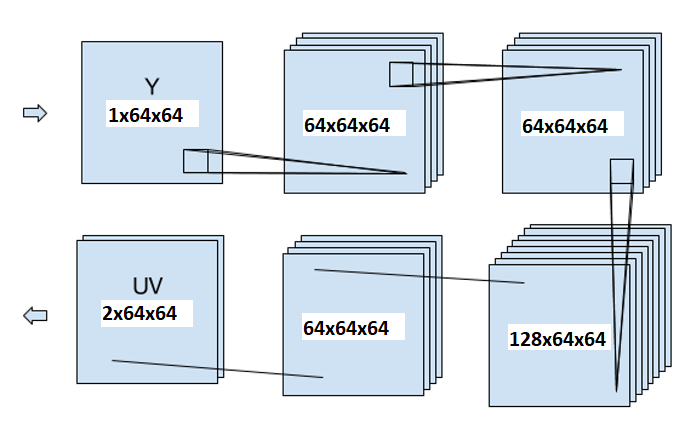
\includegraphics[width=0.5\paperwidth]{fcn}
    \caption{基线模型}
    \label{fig:fcn}
  \end{figure}

  另外一个选择是是网络层的通道数,输入的灰度图像通道为1,输出的色度图像通道为2,中间的卷积层通道数为64或128,翻倍以后再减半回来。通道数的数量在一定程度上代表了网络的最大学习能力,所以在网络使用了较多的特征通道。

  \item 变分自编码器

  变分自编码器的结构在相关工作中已经介绍过了,在本文的网络中做了一些简化,结构如图~\ref{fig:vae-2},称为编码解码模型(encoder-and-decoder)。

  \begin{figure}[H]
    \centering
    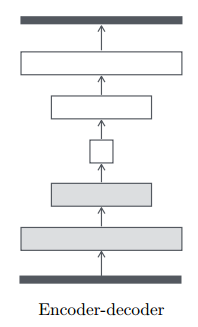
\includegraphics[width=0.2\paperwidth]{vae_2}
    \caption{编码解码模型结构示意}
    \label{fig:vae-2}
  \end{figure}

  该模型与基线模型的一点区别在于,网络卷积中图像分辨率是变化的,是一个先缩小后变大还原,即卷积与反卷积的过程,卷积的部分就是编码器,反卷积的部分就是解码器。编码器会将图像压缩到分辨率为1x1的特征向量,然后解码器将这个特征向量(即GAN模型中的随机变量)映射到色度图像。

  这个模型的详细参数如下:对于分辨率为64x64的图像,编码器包含6层卷积层及其对应的BN层和ReLU层,每个卷积层均核为4,步幅为2,边缘填充为1。每个步幅为2的卷积层都会让图像在空间上减半,特征通道上翻倍(有几个卷积层保持而不翻倍通道数)。这样图像经过编码器后得到1x1x256的特征向量。解码器包含6个反卷积层及其对应的BN层和ReLU层,每个反卷积层均核为4,步幅为2,边缘填充为1。每个步幅为2的反卷积层都会让图像在空间上翻倍,特征通道上减半(与编码器网络对应)。这样解码器输出双通道原始分辨率的图像,最后再经过一个tanh的激活函数,这在图像生成的问题上被证明是很有用的。编码器中的ReLU激活函数是LeakyReLU,而解码器中是ReLU。

  \item U-NET

  U-NET的网络结构与编码解码模型非常类似,不过在编码器与解码器的堆成卷积层(即分辨率)之间添加了捷径,即将编码器卷积层得到的特征信息连接到到解码器对应的卷积层一起输入,如图~\ref{fig:unet}所示,这样的好处是编码器中的特征有助于在解码阶段的空间信息恢复。U-NET的结构由Ronneberger~\cite{DBLP:journals/corr/RonnebergerFB15}等人2015提出,被用于生化领域的图像分割。Isola~\cite{DBLP:journals/corr/IsolaZZE16}等人在pix2pix论文中使用了这种结构,他们的任务是不同图像之间的转换,例如猫的手绘轮廓与猫的图片之间的转换,也是图像生成的范围,去掉了会丢失信息的池化层。所以本文的U-NET结构也是学习了他们的模型。

  \begin{figure}[H]
    \centering
    \subcaptionbox{原始U-NET结构\label{fig:unet_origin}}
      {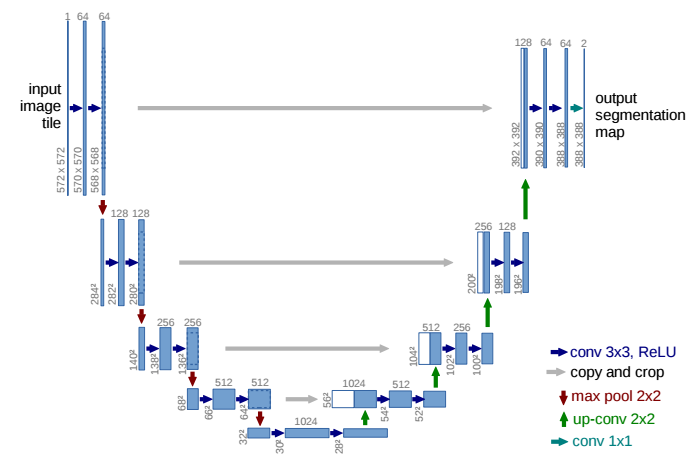
\includegraphics[width=0.45\paperwidth]{unet_origin}}
    \hspace{4em}
    \subcaptionbox{本文的U-NET结构示意\label{fig:unet}}
        {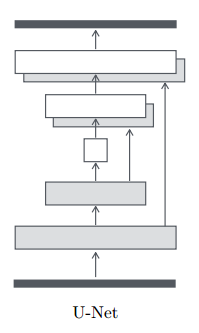
\includegraphics[width=0.15\paperwidth]{unet}}
    \caption{U-NET网络结构}
    \label{fig:unet}
  \end{figure}

  \end{enumerate}

\subsection{训练参数}
\label{sec:3-image-train}

  训练的相关参数如表~\ref{tab:3-image-train}。

  \begin{table}[ht]
    \centering
    \begin{minipage}[t]{0.8\linewidth}
    \caption{黑白图像着色GAN训练参数}
    \label{tab:3-image-train}
      \begin{tabularx}{\linewidth}{lXX}
        \toprule[1.5pt]
        {\heiti 参数名} & {\heiti 描述} & {\heiti 参数值} \\\midrule[1pt]
        image size & 图像分辨率 & 64x64 \\
        batch size & 批处理大小 & 64 \\
        epochs & 重复训练次数 & 200 \\
        ndf & 判别器第一层特征通道数 & 64 \\
        ngf & 生成器第一层特征通道数 & 64 \\
        learn rate D & 判别器学习率 & $5\times10^{-5}$ \\
        learn rate G & 生成器学习率 & $5\times10^{-5}$ \\
        D iterations & 每迭代一次生成器,判别器的迭代次数 & 5 \\
        clamp & 固定判别器参数的常数 & $\pm0.01$ \\
        optimizer & 优化函数 & RMSprop \\
        \bottomrule[1.5pt]
      \end{tabularx}
    \end{minipage}
  \end{table}

  下面对训练参数进行一些解释。图像分辨率使用了较低的64x64,因为图像分辨率增大会使得训练困难以及变慢,所以在初期均使用了较低的分辨率,以达到快速学习,验证模型可行性的目的;D iterations参数的意义是在训练的初期多进行判别器的训练,使得判别器一开始处于一个较准确的状态,从而帮助生成器学习;RMSprop优化函数是深度学习的奠基人之一Geoffrey Hinton~\cite{Tieleman2012}提出的,其目的是解决Adaptive Gradient中学习速率趋向于0的问题。

  另外,我们已经知道生成器的输入是单通道的灰度图像,使用的是YUV色彩空间的Y通道,输出是双通道的色度图像,使用的是YUV中的UV通道,训练图像的YUV值均归一化到[-1,1]。

\section{黑白视频着色}
\label{sec:3-video-color}

  在2D模型上验证了可行性后,就要将模型扩展到3D上处理黑白视频着色问题。本文使用GAN做视频着色的想法来源于3D-GAN的论文~\cite{DBLP:conf/nips/0001ZXFT16}。这篇论文的目的是从一个随机变量生成3D像素空间的模型,有趣的是他们还训练了一个生成器为VAE模型的网络,用于将2D图片转换为3D模型。对于本文的问题而言,从2D扩展到3D不是在空间上,而是在时间上。另外本文并不是将整个视频作为3D数据输入,因为每个视频的长短不一样,网络无法处理帧数不一样的各个视频,所以本文采取等间距采样获取一定数量的关键帧,将这部分关键帧通过网络着色后再用非学习的方法给剩余未着色的帧着色。

  本文的3D着色模型判别器与生成器均分别从2D对应的模型扩展而来,下面介绍本文的网络结构以及训练参数。

\subsection{判别器网络}
\label{sec:3-video-dnet}
  
  判别器网络直接从图片着色网络扩展而来:使用3D的卷积函数和3D的BN函数;之前的卷积核是2D的,大小为4x4,扩展到3D后,大小为4x4x4,同样步幅由2x2变为2x2x2,边缘填充由1x1变为1x1x1。卷积层及其对应的BN层和LeakyReLU层还是4层。最后经过一个卷积核为1x4x4的卷积层得到判别器给出的图像为真实的概率。卷积核大小为1x4x4的原因在第\ref{sec:3-video-train}节解释。
  
\subsection{生成器网络}
\label{sec:3-video-gnet}

  本文的生成器网络选择从U-NET扩展到3D,因为在黑白图像着色阶段被证明U-NET是最好的结构。这个网络的结构如下:输入64x64x8的单通道图像序列,经过6层卷积核4、步幅2、边缘填充1的卷积层及其对应的BN层和LeakyReLU层,得到1x1x1x256的特征向量,然后经过6层卷积核卷积核4、步幅2、边缘填充1的反卷积层,得到64x64x8的双通道图像,再经过一层tanh激励函数后得到输出色度图像序列。其中在解码的反卷积阶段,前面对应的编码卷积层的输出特征都添加到反卷积输入中,以帮助空间信息的恢复。

\subsection{训练参数}
\label{sec:3-video-train}

  黑白视频着色训练的相关参数如表~\ref{tab:4-video-train}。

  \begin{table}[h]
    \centering
    \begin{minipage}[t]{0.8\linewidth}
    \caption{黑白视频着色GAN训练参数}
    \label{tab:4-video-train}
      \begin{tabularx}{\linewidth}{lXX}
        \toprule[1.5pt]
        {\heiti 参数名} & {\heiti 描述} & {\heiti 参数值} \\\midrule[1pt]
        image size & 图像分辨率 & 64x64 \\
        batch size & 批处理大小 & 64 \\
        frame size & 单视频截取帧数 & 8 \\
        epochs & 重复训练次数 & 200 \\
        ndf & 判别器第一层特征通道数 & 64 \\
        ngf & 生成器第一层特征通道数 & 64 \\
        learn rate D & 判别器学习率 & $5\times10^{-5}$ \\
        learn rate G & 生成器学习率 & $5\times10^{-5}$ \\
        D iterations & 每迭代一次生成器,判别器的迭代次数 & 5 \\
        clamp & 固定判别器参数的常数 & $\pm0.01$ \\
        optimizer & 优化函数 & RMSprop \\
        \bottomrule[1.5pt]
      \end{tabularx}
    \end{minipage}
  \end{table}

  视频着色与图像着色的差别就是多了一个单视频截取帧数的参数,在这里本文取值为8,即对于训练数据集中的每个视频,等间距的取出8帧图像代表这个视频,输入给着色网络。帧数上的分辨率小于图像空间上的分辨率就会导致一个问题,即使用卷积核为4的卷积时,帧数维度会先于空间维度压缩到大小为1,继续卷积会出现问题,所以在帧数维度压缩到1后,在帧数维度上的卷积层,设置为卷积核为3,步幅为1,边缘填充为1,这样可以保持帧数维度上1的分辨率不变。这也是本文在判别器最后一层卷积层使用了1x4x4的卷积核的原因。

\section{关键帧平滑与非关键帧着色}
\label{sec:3-other-algorithm}

  在这一节中,将介绍本文用于对着色后的关键帧在空间和时间上平滑的算法,以及得到关键帧平滑着色后用于给非关键帧着色的算法。

  由于一些原因,本文最后的视频着色并没有使用第~\ref{sec:3-video-color}节中的3D模型,而使用的第~\ref{sec:3-image-color}中的2D着色模型,本文将在第~\ref{sec:3-experiment}节中给出解释。

  所以整体算法的流程如下:

  \begin{enumerate}
    \item 对于输入黑白视频,等间距提取出关键帧;
    \item 用训练好的二维GAN网络的生成器网络给关键帧着色;
    \item 分别对每一个关键帧做空间平滑处理;
    \item 综合所有关键帧,依次对其做时间平滑处理;
    \item 利用得到的关键帧颜色对非关键帧进行着色;
    \item 输出着色后的视频。
  \end{enumerate}

\subsection{空间平滑算法}
\label{sec:3-spatial-smooth}

  对于一张黑白图像而言,现在的基于学习的自动着色算法输出的着色或多或少都会存在一些空间上的不连续,很容易被人识别出来,所以需要做一个空间平滑的处理。

  本文的空间平滑算法具体如下:输入待平滑彩色图像,遍历其所有像素;对于每个像素,搜索其邻近的像素(在实验中本文取的以该像素为中心的5x5的patch),如果邻近像素的灰度值与该像素的灰度值差在一定范围内(YUV色彩空间中的Y值),则邻近像素视为与原像素属于同物体;搜索完邻近像素后,将所有被视为原像素同物体的像素的色度值取平均值(YUV色彩空间中的UV值),作为该像素新的色度值。

  算法伪代码如下。

  \begin{algorithm}[H]
  \label{algo:5-spatial-smooth}
    \caption*{空间平滑算法}
    \begin{algorithmic}[1]
      \Require $Y$, $UV$
      \Ensure  $UV$
      \Function{spatial smooth}{}
        \For {pixel $p \in Y$}
          \State $\Omega = \phi$
          \For {pixel $\|p^{'} - p\| <= 2$}
            \If {$\|Y(p) - Y(p^{'})\| < \epsilon$}
              \State $\Omega = \Omega \cup p^{'}$
            \EndIf
          \EndFor
          \State $UV(p) = mean(UV(\Omega))$
        \EndFor
      \EndFunction
    \end{algorithmic}
  \end{algorithm}


\subsection{时间平滑算法}
\label{sec:3-temporal-smooth}

  将关键帧依次给着色网络着色病不能保证视频颜色在时间上的稳定性,这一点本文在第~\ref{sec:3-experiment}节中进行了实验。所以在得到每个关键帧的独立着色后,需要对这一系列关键帧的颜色进行平滑,使它们保持一致性。关键帧的稳定是非关键着色稳定的前提,也是视频颜色稳定的前提。

  本文的时间平滑算法如下:输入一系列按时间排序的关键帧彩色图像,设有K帧,对于每个关键帧,做如下处理:用Gunnar~\cite{DBLP:conf/scia/Farneback03}等人2003年提出的光流算法计算关键帧F其与其他$(K-1)$个关键帧之间的光流,这样对关键帧$F$中的每个像素$p$而言,可以找到其在其他关键帧中的$(K-1)$个对应像素,去掉不在图像范围内的,去掉像素灰度值与像素$p$灰度值的差超过一定值的像素,取剩下符合要求像素的色度平均值,作为像素$p$平滑后的色度值。这样对于每个关键帧的每个像素,它们的色度都是比较相近的,排除了着色网络在某些帧会给出与一般情况差别较大的误差。

  算法伪代码如下。

  \begin{algorithm}[H]
  \label{algo:5-temporal-smooth}
    \caption*{时间平滑算法}
    \begin{algorithmic}[1]
      \Require $Ys$, $UVs$
      \Ensure  $UVs$
      \Function{temporal smooth}{}
        \For {$Y_i \in Ys$}
          \For {$Y_j \in Ys$}
            \State $flow = \textbf{GunnarOpticalFlow}(Y_i, Y_j)$
            \For {$p \in Y_i$}
              \State $p^{'} = p + flow(p)$
              \If {$\|Y_i(p) - Y_j(p^{'})\| < \epsilon$}
                \State $\Omega_p = \Omega_p \cup UV_j(p^{'})$
              \EndIf
            \EndFor
          \EndFor
          \For {$p \in Y_i$}
            \State $UV_i(p) = mean(\Omega_p)$
          \EndFor
        \EndFor
      \EndFunction
    \end{algorithmic}
  \end{algorithm}

\subsection{非关键帧着色算法}
\label{sec:3-interframe-color}

  在得到所有关键帧的平滑着色后,就要将关键帧的色度传递到剩余非关键帧。本文的算法采取相邻帧迭代传递色度的方法,即从已着色的关键帧$F_{nk}$开始,用它的颜色传递到它的下一帧$F_{nk+1}$(非关键帧);当第$F_{nk+1}$帧着色完成时,它又可以作为第$F_{nk+2}$帧的参考帧,将颜色传递给第$F_{nk+2}$帧;重复这个过程,当着色到下一个关键帧$F_{n(k+1)}$时,又可以从这个关键帧开始下一轮颜色传递。

  本文的色彩传递算法具体如下:设前一帧参考帧为$F_p$,待着色的帧为$F_c$,首先计算两帧之间的光流,对于$F_c$中的待着色像素$p_c$而言,在$F_p$中可找到光流对应的像素$p_c^{'}$,另外还有$F_p$中与像素$p_c$同位置的$p_p$,取$p_p$周围3x3的patch的像素$N(p_p)$,然后在像素集合${p_c^{'},N(p_p)}$中找与像素$p_c$灰度值差最小的像素$r$,即

  \begin{equation}
  \label{equ:5-interframe}
    r = \mathop{\arg\min}_{p \in \{p_c^{'},N(p_p)\}} \|Y_c(p_c) - Y_p(p)\|^2
  \end{equation}

  然后取$r$的色度值作为$p_c$的色度值。对$F_c$中的每个像素做如上操作即可完成帧$F_c$的着色。

  算法伪代码如下。

  \begin{algorithm}[H]
  \label{algo:5-interframe}
    \caption*{非关键帧着色算法}
    \begin{algorithmic}[1]
      \Require $Y_c$, $Y_p$, $UV_p$
      \Ensure  $UV_c$
      \Function{color flow}{}
        \State $flow = \textbf{GunnarOpticalFlow}(Y_c, Y_p)$
        \For {$p_c \in Y_c$}
          \State $p_c^{'} = p_c + flow(p_c)$
          \State $\Omega = \{p_c^{'}\}$
          \For {$\|p - p_c\| < \epsilon$}
            \State $\Omega = \Omega \cup p$
          \EndFor
          \For {$p \in \Omega$}
            \If {$\|Y_p(p) - Y_c(p_c)\| < min$}
              \State $r = p$
            \EndIf
          \EndFor
          \State $UV_c(p_c) = UV_p(r)$
        \EndFor
      \EndFunction
    \end{algorithmic}
  \end{algorithm}

\section{实验及结果}
\label{sec:3-experiment}
  
  实验对比一节依然分为图像着色与视频着色分别讨论。

\subsection{黑白图像着色}
\label{sec:3-image-color-exp}

  对于图像着色,本文在三个数据集上进行了实验,与两种目前效果最好的学习算法进行了对比。

  三个数据集分别是:LSUN-CHURCH~\cite{DBLP:journals/corr/YuZSSX15},是一个教堂图片的数据集,数据规模为12w训练集,300验证集;CIFAR-10~\cite{CIFAR-10},是一个包含10类图片的数据集,数据规模为5w训练集,1w测试集;IMAGE-NET~\cite{DBLP:journals/ijcv/RussakovskyDSKS15},是一个大型的分类数据集,包含1000类物体,本文采用了它的部分子集,数据规模为28w训练集,1w测试集。

  进行对比的两个图像自动着色算法是Iizuka等人Siggraph2016的\inlinecite{IizukaSIGGRAPH2016},与Zhang等人ECCV2016的\inlinecite{zhang2016colorful}。

  本文选择均方误差(MSE)作为评价标准,即以网络着色结果与真是彩色图像之间的像素均方差作为误差。表~\ref{tab:6-image-error}给出了误差对比。需要注意的是,本文的网络是在三个数据集下分别独立的,即Ours$_l$指的是在LSUN-CHURCH下训练的本文的网络,Ours$_c$与Ours$_i$以此类推;另外,均方误差值取的是64x64分辨率图片的像素误差和,且像素UV值已归一化到[-1,1]。

  \begin{table}[H]
    \centering
    \begin{minipage}[t]{0.8\linewidth}
    \caption{黑白图像着色均方误差对比}
    \label{tab:6-image-error}
      \begin{tabularx}{\linewidth}{|l|X|X|X|}
        \hline
        \multirow{2}*{\diagbox[width=6em]{\heiti 方法}{\heiti 数据集}} & \multirow{2}*{LSUN-CHURCH} & \multirow{2}*{CIFAR-10} & \multirow{2}*{IMAGE-NET} \\
         & & & \\\hline
        Ours$_l$ & 127.1 & - & - \\\hline
        Ours$_c$ & - & 347.9 & - \\\hline
        Ours$_i$ & - & - & 174.5 \\\hline
        Zhang    & 151.8 & 367.5 & 282.8 \\\hline
        Iizuka   & \textbf{86.7}  & \textbf{117.2} & \textbf{127.6} \\\hline
      \end{tabularx}
    \end{minipage}
  \end{table}

  从表~\ref{tab:6-image-error}进行方法的纵向对比,可以发现本文的生成对抗模型总体来说表现比Zhang~\cite{zhang2016colorful}等人的卷积神经网络好,但与Iizuka~\cite{IizukaSIGGRAPH2016}等人的卷积神经网络相比还差距较大;在本文的方法内部进行数据集间的横向对比可以发现:当在只有一类物体的LSUN-CHURCH数据集上时,本文的均方误差较小,当在物体种类较多的IMAGE-NET上训练时,误差变大;当图像分辨率变小时(CIFAR-10的图像分辨率只有32x32),误差也会明显增大。

  图~\ref{fig:lsun-compare},图~\ref{fig:cifar-compare},图~\ref{fig:imagenet-compare}分别给出了LSUN-CHURCH、CIFAR-10、IMAGE-NET数据集下本文的网络着色与真实图像的对比。

  \begin{figure}[ht]
    \centering
    \subcaptionbox{本文网络的着色结果\label{fig:lsun_fake}}
      {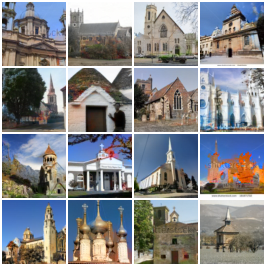
\includegraphics[width=0.3\paperwidth]{lsun_fake}}
    \hspace{2em}
    \subcaptionbox{真实彩色图像\label{fig:lsun_real}}
        {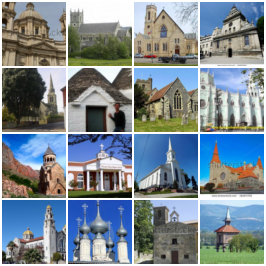
\includegraphics[width=0.3\paperwidth]{lsun_real}}
    \caption{LSUN-CHURCH数据集测试结果}
    \label{fig:lsun-compare}
  \end{figure}

  \begin{figure}[ht]
    \centering
    \subcaptionbox{本文网络的着色结果\label{fig:cifar_fake}}
      {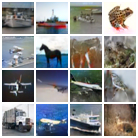
\includegraphics[width=0.3\paperwidth]{cifar_fake}}
    \hspace{2em}
    \subcaptionbox{真实彩色图像\label{fig:cifar_real}}
        {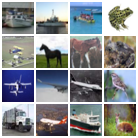
\includegraphics[width=0.3\paperwidth]{cifar_real}}
    \caption{CIFAR-10数据集测试结果}
    \label{fig:cifar-compare}
  \end{figure}

  \begin{figure}[ht]
    \centering
    \subcaptionbox{本文网络的着色结果\label{fig:imagenet_fake}}
      {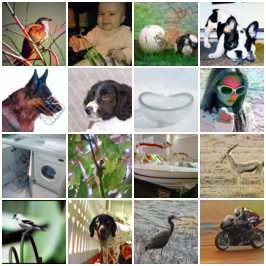
\includegraphics[width=0.3\paperwidth]{imagenet_fake}}
    \hspace{2em}
    \subcaptionbox{真实彩色图像\label{fig:imagenet_real}}
        {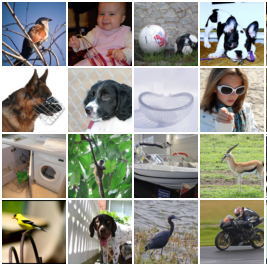
\includegraphics[width=0.3\paperwidth]{imagenet_real}}
    \caption{IMAGE-NET数据集测试结果}
    \label{fig:imagenet-compare}
  \end{figure}

  从这些结果中分析得出这样的结论:GAN处理着色问题相比CNN更逊色。图像风格转换的任务已经被证明非常适合GAN模型,Zhu~\cite{DBLP:journals/corr/ZhuPIE17}等人最新的网络结构cycleGAN在做两种风格图片转换的任务上取得了很好的效果,比如油画风格与照片写实风格之间的互相转换。着色问题也可以看作一个风格转换问题(黑白风格到彩色风格的转换),但相比前者,着色问题里图像的域更大:前者可能只是莫奈的油画风格与真实照片的转换,而着色中的图像包含了多种物体的多种可能颜色,对于一种物体有效的着色对于另一种物体就不行。所以在单一物体的LSUN-CHURCH数据集上表现更好,而在多物体的CIFAR-10与IMAGE-NET的数据集上就表现更差。

\subsection{黑白视频着色}
\label{sec:3-video-color-exp}

  对于视频着色,本文在UCF11数据集上进行了实验,与之前的最先进的自动黑边图像着色算法直接应用于视频进行了对比。

  UCF11~\cite{DBLP:conf/cvpr/LiuLS09}是一个人体动作识别的数据库,包含11类人类不同运动的短视频共2000段。在这个数据集上使用本文第~\ref{sec:3-video-color}节中的3D模型时,生成器无法向真实图像进行学习,结果是着色的关键帧一直是非常暗淡没有什么色彩,在反复调试后也不能得到有意义的结果,图~\ref{fig:3d_result}就是本文的3D网络着色结果。于是只好暂时放弃用3D模型着色的想法,使用2D的GAN模型给关键帧着色。

  \begin{figure}[H]
    \centering
    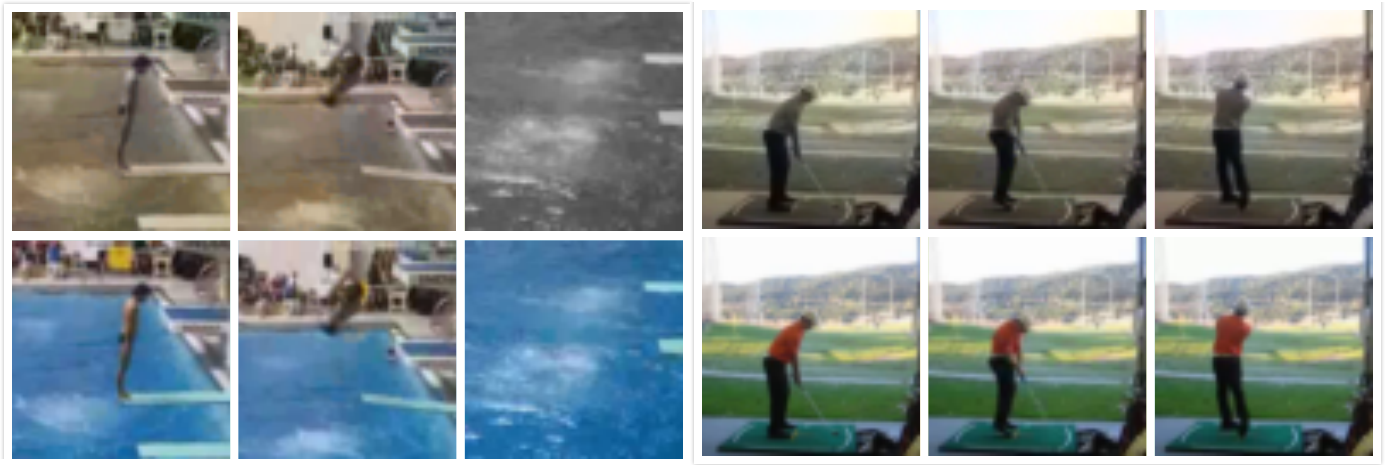
\includegraphics[width=0.7\paperwidth]{3d_result}
    \caption[3D网络着色结果]{3D网络的着色结果。第一行是本文的着色,第二行是真实视频帧;前三列来自一个跳水视频,后三列来自一个高尔夫视频}
    \label{fig:3d_result}
  \end{figure}

  使用2D网络对视频着色的流程在第~\ref{sec:3-other-algorithm}节已经介绍过了。训练时本文使用UCF11中的2000个视频,每个视频等间距取采样帧作为训练图像数据,共约2w的训练集,测试集有约100个独立的视频。

  图~\ref{fig:2d_result}是本文的2D网络着色结果。

  \begin{figure}[H]
    \centering
    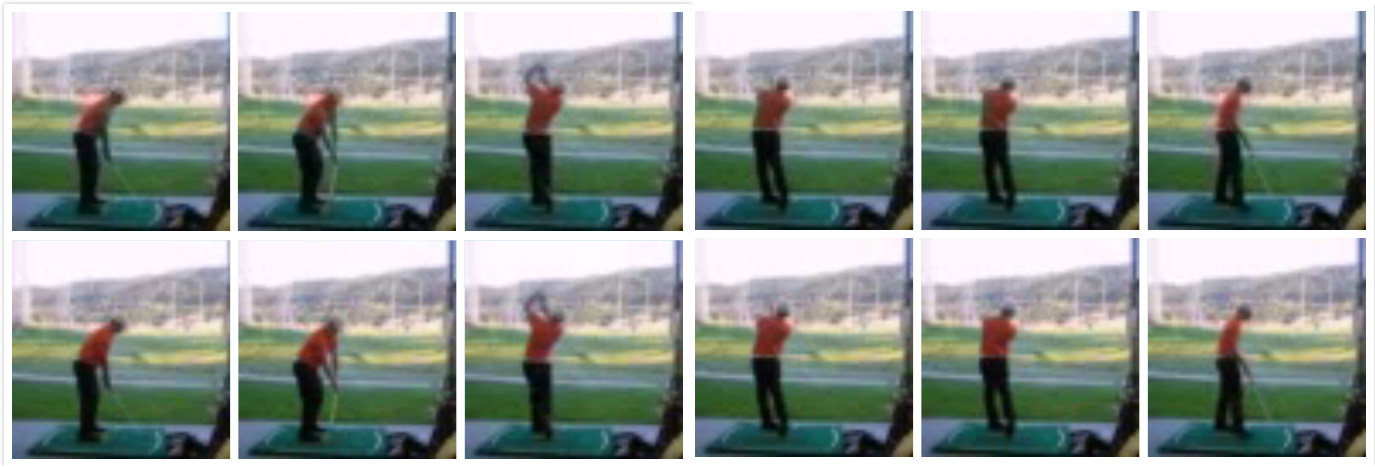
\includegraphics[width=0.7\paperwidth]{2d_result}
    \caption[2D网络着色结果]{3D网络的着色结果。第一行是我们的着色视频帧,第二行是真实视频帧}
    \label{fig:2d_result}
  \end{figure}

  另外单帧着色带来的时间空间不稳定性通过本文第~\ref{sec:3-other-algorithm}节中的平滑可以解决,这一点可以从图~\ref{fig:2d_result_compare}中看出。

  \begin{figure}[H]
    \centering
    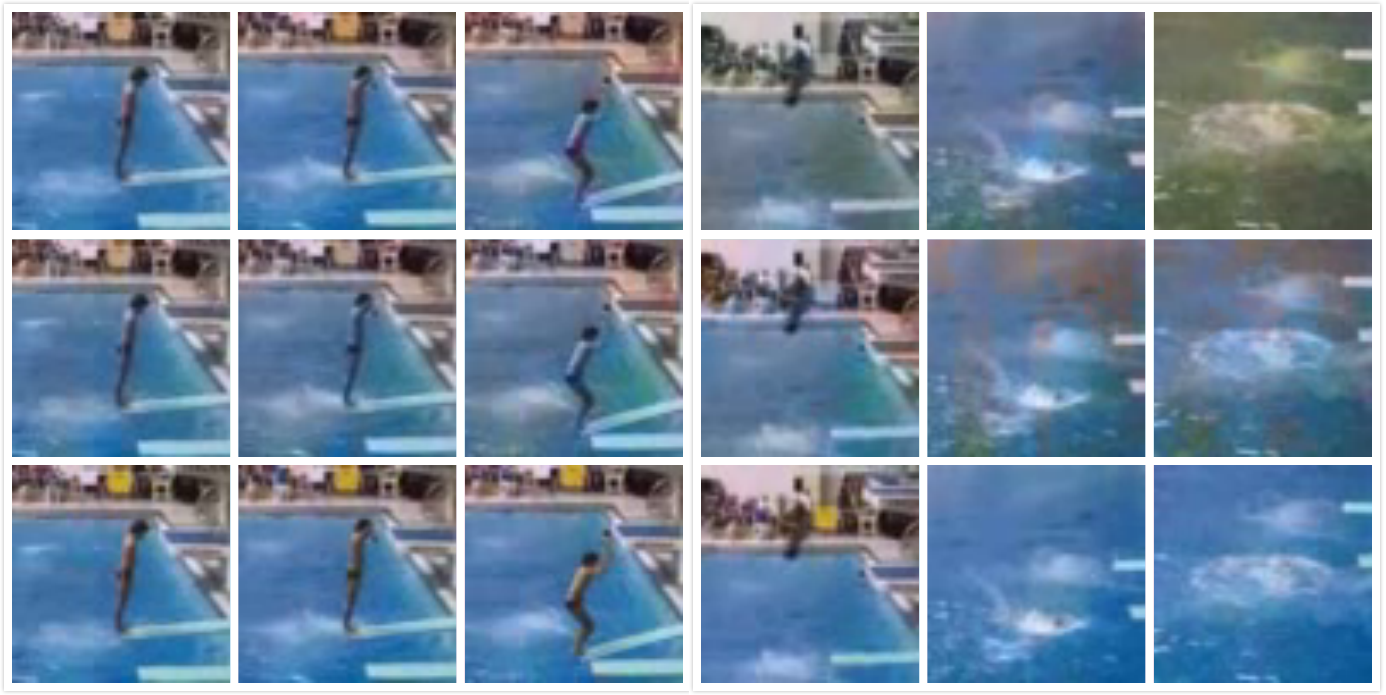
\includegraphics[width=0.7\paperwidth]{2d_result_compare}
    \caption[时空平滑效果比较]{时空平滑效果比较。第一行是本文直接使用2D网络对每一帧着色的结果,第二行是本文用2D网络对关键帧着色然后进行时空平滑处理的结果,第三行是真实视频帧}
    \label{fig:2d_result_compare}
  \end{figure}

  表\ref{tab:3-video-error}给出了我们的方法与Iizuka和Zhang方法的量化对比。在着色准确度方面,我们计算了测试视频与真实视频每帧像素之间的均方误差;在时间一致性方面,我们计算了测试视频着色结果每对相邻帧之间的均方误差。可以看到,我们的着色准确度相比另外两个方法要好,而时间一致性方面,Iizuka方法的误差最小,甚至比真实视频的误差还低,经验证发现Iizuka方法对视频的着色效果不太好,着色后的视频与初始的灰度视频差不多,所以在时间连续性误差上较小。综合两项,本文的方法在UCF11视频数据集上表现比其他两个方法要好。

  \begin{table}[H]
    \centering
    \begin{minipage}[t]{0.8\linewidth}
    \caption{黑白视频着色误差对比}
    \label{tab:3-video-error}
      \begin{tabularx}{\linewidth}{|l|X|X|}
        \hline
        \multirow{2}*{\diagbox[width=8em]{\heiti 方法}{\heiti 评测方法}} & \multirow{2}*{均方误差} & \multirow{2}*{时间连续性误差} \\
         & & \\\hline
        Ground Truth & 0 & 2.55 \\\hline
        Ours & \textbf{161.01} & 6.14 \\\hline
        Zhang & 757.75 & 26.03 \\\hline
        Iizuka & 499.17 & \textbf{1.59} \\\hline
      \end{tabularx}
    \end{minipage}
  \end{table}

  另外本文也用图像着色中LSUN-CHURCH教堂数据集训练的网络给大礼堂进行了着色,如图~\ref{fig:extra_result}。

  \begin{figure}[H]
    \centering
    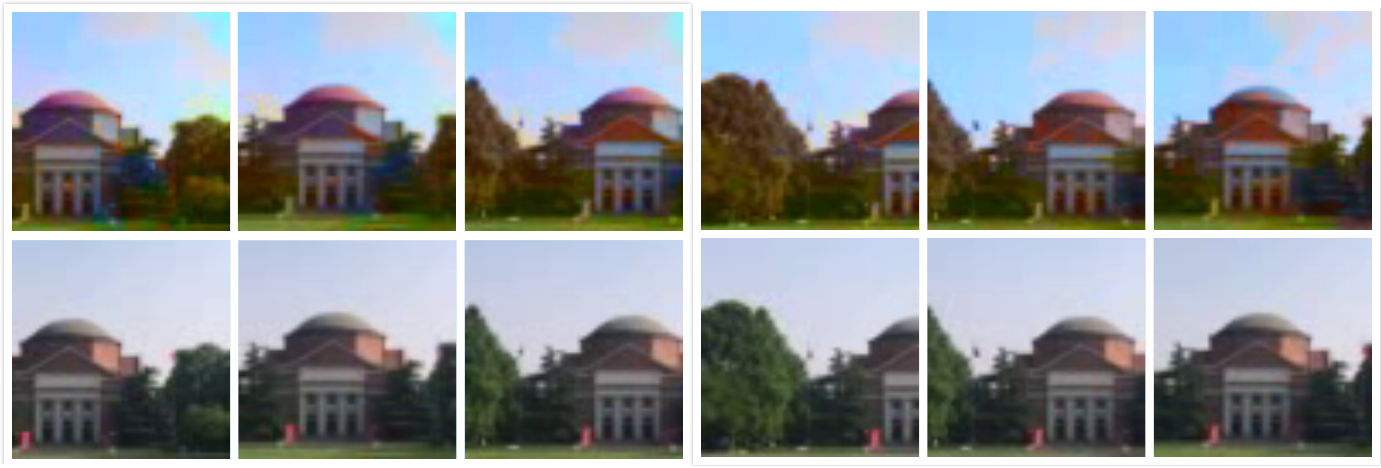
\includegraphics[width=0.7\paperwidth]{extra_result}
    \caption[大礼堂着色效果]{大礼堂着色效果。第一行是本文的着色结果,第二是真实拍摄的视频}
    \label{fig:extra_result}
  \end{figure}

  \begin{figure}[H]
    \centering
    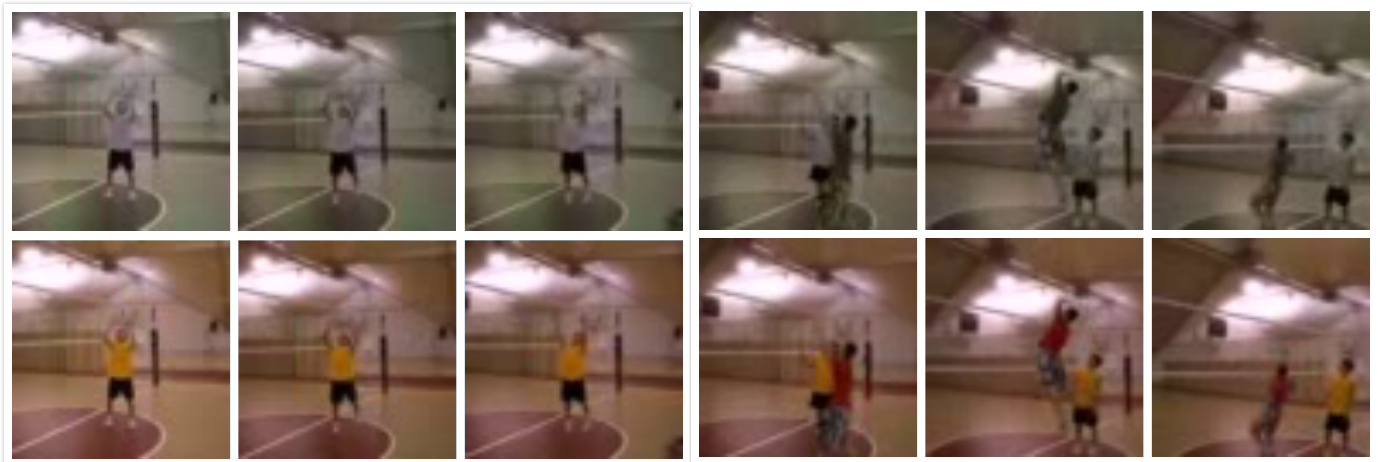
\includegraphics[width=0.7\paperwidth]{failure_case}
    \caption[失败案例]{失败案例。第一行是本文的着色结果,第二是真实拍摄的视频}
    \label{fig:failure_case}
  \end{figure}  

  不过在UCF11数据集下也有一些失败的案例,如图~\ref{fig:failure_case},通常的体现是没有什么色彩。分析原因为:当视频场景中物体动作幅度不是很大时,着色能有较好的效果(如高尔夫击球),相反动作幅度较大时(如排球扣球),网络便不那么稳定;场景的特征颜色较明显时(如跳水中的蓝色),着色结果很理想,而场景没有明显的颜色特征时,网络变只能给出灰褐色的平凡结果。





  